\documentclass{article}
%\usepackage[pdftex]{} % for pdf features
\usepackage{thumbpdf} % for thumbnails
%\usepacakge{tex4ht}
\usepackage[pdftex,
	pdftitle={Riddling},
	pdfauthor={Mark Veltzer},
	pdfsubject={A collection of riddles},
	pdfkeywords={riddling, riddles, math, mathematics, geometry, combinatorics, Mark Veltzer, veltzer, Veltzer},
	pdfproducer={Mark Veltzer <mark.veltzer@gmail.com>},
	]{hyperref}
\pdfminorversion=5
\pdfoutput=1
\pdfcompresslevel=0
%\usepackage{pdftricks}
%\usepackage{pst-all}
% if you use the following package straight latex running (not via pdflatex), will not work...
\usepackage{pst-pdf}
%\usepackage{auto-pst-pdf}
%	colorlinks=true,
%	urlcolor=rltblue, % \href{...}{...} external (URL)
%	filecolor=rltgreen, % \href{...} local file
%	linkcolor=rltred, % \ref{...} and \pageref{...}
%	pagebackref,
%	pdfpagemode=UseNone,
%	bookmarksopen=true]{hyperref} % needed for sketch
%\definecolor{rltred}{rgb}{0.75,0,0}
%\definecolor{rltgreen}{rgb}{0,0.5,0}
%\definecolor{rltblue}{rgb}{0,0,0.75}
%\usepackage{amsmath,color,thumbpdf,html,hyperref}
%\usepackage{pst-barcode,pstricks-add}

% these are the packages that we actually use
%\usepackage{hyperref} % for hyperlinks
%\usepackage{color} % for colors (creates errors when applied with pdftex option)
\usepackage{amsmath} % for math (does not pdftex option)
\usepackage{amssymb} % for math symbols (does not pdftex option)
%\usepackage{pstricks} % for sketch with pstricks support (default for sketch)
\usepackage{tikz} % for sketch with tikz (does not pdftex option)

\title{Riddles}
\author{Mark Veltzer}
\date{\today}

\begin{document}

\maketitle

\tableofcontents

\section{Rational points on a circle (Calculus)}
Could there be a circle on the plane where only one point has rational co-ordinates? A point $p=(x,y)$ has rational co-ordinates iff $x,y\in\mathbb{Q}$. What about a sphere? Are there circles with more than one rational point? Are there circles with infinite rational points? Can you find a circle with exactly $n$ rational points on it for each $n\in\mathbb{N}$?

\subsection{Solution}
Yes, there could. Consider the circle: $(x-r)^2+y^2=r^2$ for some irrational $r$.
$(0,0)$ is a point on this circle and is rational. But from the equation it follows
that: $x^2-2xr+r^2+y^2=r^2$ or $x^2+y^2=2xr$ or $r=(x^2+y^2)/2x$. If there
was a rational solution to this equation where $x\ne0$ then it would follow that
$r$ is rational since it is the result of multiplication, division, addition and subtration
of rational numbers and this is a contradiction. This means this equation can only
have rational solutions for $x=0$. If $x=0$ then $r^2+y^2=r^2$ and so $y=0$ and so
$(0,0)$ is the only such solution.

Same solution applies to a sphere: $(x-r)^2+y^2+z^2=r^2$ for some irrational $r$.
In this case: $r=(x^2+y^2+z^2)/2x$. Which means that for $x\ne0$ any rational soultion would imply a rational $r$.
$(0,0,0)$ is therefor the only rational solution.

Yes, there are circles with more than one rational point. Take $x^2+y^2=2$ which is the circle whose
center is at $(0,0)$ and whose radius is $\sqrt{2}$. The points $(1,1),(-1,1),(1,-1),(-1,-1)$ are four rational
points which are on this circle.

Yes, there are circles with infinite rational points (TODO).

What about for each $n\in\mathbb{N}$? (TODO).

\section{Always lead in election (Combinatorics)}
An election was voted a perfect tie (even number of electors) and was decided by way of putting
all the votes into a hat, mixing them uniformly and counting them one by one. What is the chance
that one of the candidates was leading during the entire counting process?

\subsection{Solution}
The question could be rephrased as how many graphs that go either one step up or one step down (lets call those binary graphs) do not go down below zero out of the set of all graphs that go from zero to zero. At first lets note that in the following solution $n$ is even and so there is no problem with $n/2$. A first observation is that the set of all graphs going from 0 to 0 in $n$ steps is ${n \choose n/2}$.

Let's try to count the graphs that tip below 0. Every graph that tips below 0 will reach -1 at one or more points. Lets find the first place where the graph reaches -1. From that point on the graph climbs one more than it descends since it finally reaches 0. Lets flip it from that point on - meaning switch every climb with descent and every descent with a climb. Now the graph descends one more than it climbs and since it starts from that point at height -1 then it now reaches a height -2 at $n$ instead of the original 0.

The main proposition is that \emph{every} graph which travels from 0 to -2 correspons with a \emph{1-1 correspondance} to graphs that travel from 0 to 0 and reach -1 at some point (convince yourself
of this).

If this is so then the number of graphs that go from 0 to -2 is ${n \choose n/2+1}$ since we need to
choose points at which the graph will go down and we have $n/2+1$ descends. If so then the number of
graphs that do not reach -1 is:

${n \choose n/2} - {n \choose n/2+1} = \frac{(n)!}{(n/2+1)!(n/2)!} = \frac{1}{n/2+1}{n \choose n/2}$.

And now back to the original question "What is the chance that one of the candidates was leading during the entire counting process?". Lets divide the latter result with the former and get:

$\frac{1}{n/2+1}{n \choose n/2} / {n \choose n/2} = \frac{1}{n/2+1}$

The result is all about \htmladdnormallink{Catalan numbers}{http://en.wikipedia.org/wiki/Catalan_number}
and \htmladdnormallink{Bertrand's ballot theorem}{http://en.wikipedia.org/wiki/Bertrand\%27s_ballot_theorem}.

One of the interesting results of this question is that ${n \choose n/2}$ is divisible by $n/2+1$. One reason
is the argument stated above but a more direct number theory based argument may be found. A more general result
relating to ${n \choose k}$ for any $k$ may also be obtained (TODO).

\section{Four Coke bottles on a table (Geometry)}
Arrange four Coke bottles on a table so that the distances between each pair of caps will be the same. Assume that
you can make a Coke bottle stand on it's head (this is a pretty strong hint!, maybe I should remove it ?!?). The length
or height of each bottle is ${h}$.

\subsection{Solution}
There are two solutions:

The first solution is to put the bottles in a square where the side of the square is the length of the bottle. Bottles
next to each other will stand \emph{in reverse} (if the first is on it's head the the second will stand straight).

\begin{center}
% Sketch output, version 0.3 (build 7d, Wed May 2 06:36:52 2012)
% Output language: PGF/TikZ,LaTeX
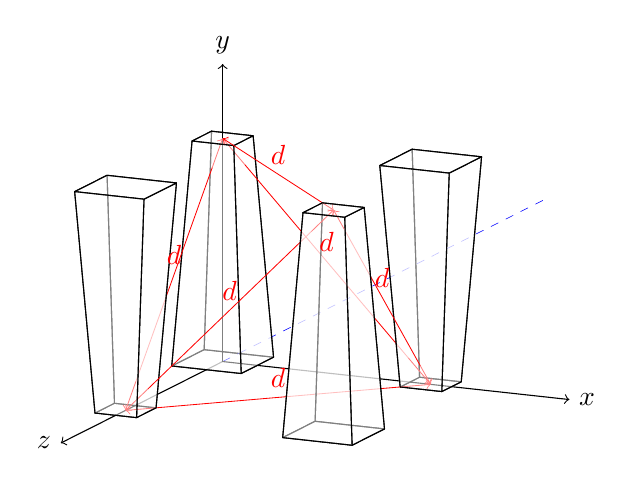
\begin{tikzpicture}[line join=round]
\draw[arrows=-](-2.055,-1.034)--(-2.261,-1.138);
\filldraw[fill opacity=0.5,fill=white](-2.29,-.883)--(-2.701,-1.09)--(-1.82,-1.186)--(-1.409,-.979)--cycle;
\draw[line width=.2pt,draw=blue,dashed](-1.85,-.931)--(2.055,1.034);
\filldraw[fill opacity=0.5,fill=white](-1.409,-.979)--(-2.29,-.883)--(-2.196,1.891)--(-1.668,1.833)--cycle;
\filldraw[fill opacity=0.5,fill=white](-2.29,-.883)--(-2.701,-1.09)--(-2.443,1.767)--(-2.196,1.891)--cycle;
\draw[line width=.2pt,draw=blue,dashed](-2.055,-1.034)--(-1.85,-.931);
\draw[arrows=-](-2.055,-1.034)--(-1.615,-1.083);
\draw[line width=.3pt,arrows=<-,draw=red](-2.055,1.8)--(-1.772,1.465);
\filldraw[fill opacity=0.5,fill=white](-1.82,-1.186)--(-1.409,-.979)--(-1.668,1.833)--(-1.914,1.709)--cycle;
\draw[arrows=-](-2.055,-1.034)--(-2.055,1.8);
\filldraw[fill opacity=0.5,fill=white](.975,-1.291)--(.728,-1.415)--(.2,-1.357)--(.446,-1.233)--cycle;
\draw[arrows=-](-1.615,-1.083)--(.323,-1.295);
\draw[line width=.3pt,arrows=->,draw=red](-2.187,1.43)--(-2.055,1.8);
\filldraw[fill opacity=0.5,fill=white](-2.701,-1.09)--(-1.82,-1.186)--(-1.914,1.709)--(-2.443,1.767)--cycle;
\filldraw[fill opacity=0.5,fill=white](-2.196,1.891)--(-2.443,1.767)--(-1.914,1.709)--(-1.668,1.833)--cycle;
\draw[arrows=-](-2.261,-1.138)--(-3.165,-1.593);
\draw[arrows=->](-2.055,1.8)--(-2.055,2.745);
\draw[line width=.3pt,arrows=<-,draw=red](-2.055,1.8)--(-1.914,1.709);
\draw[line width=.3pt,arrows=-,draw=red](-1.772,1.465)--(.304,-.989);
\filldraw[fill opacity=0.5,fill=white](-.059,1.455)--(.352,1.662)--(.446,-1.233)--(.2,-1.357)--cycle;
\filldraw[fill opacity=0.5,fill=white](.352,1.662)--(1.233,1.566)--(.975,-1.291)--(.446,-1.233)--cycle;
\draw[line width=.3pt,arrows=-,draw=red](-3.156,-1.285)--(-2.187,1.43);
\draw[line width=.3pt,arrows=-,draw=red](-1.914,1.709)--(-.787,.981);
\draw[arrows=-](.323,-1.295)--(.851,-1.353);
\filldraw[fill opacity=0.5,fill=white](1.233,1.566)--(.822,1.359)--(.728,-1.415)--(.975,-1.291)--cycle;
\draw[line width=.3pt,arrows=->,draw=red](.304,-.989)--(.587,-1.324);
\draw[line width=.3pt,arrows=<-,draw=red](.587,-1.324)--(.2,-1.357);
\draw[line width=.3pt,arrows=<-,draw=red](.587,-1.324)--(.455,-1.087);
\filldraw[fill opacity=0.5,fill=white](1.233,1.566)--(.822,1.359)--(-.059,1.455)--(.352,1.662)--cycle;
\draw[arrows=->](.851,-1.353)--(2.349,-1.517);
\filldraw[fill opacity=0.5,fill=white](.822,1.359)--(-.059,1.455)--(.2,-1.357)--(.728,-1.415)--cycle;
\filldraw[fill opacity=0.5,fill=white](-2.901,-1.622)--(-3.148,-1.746)--(-3.676,-1.688)--(-3.429,-1.564)--cycle;
\draw[line width=.3pt,arrows=-,draw=red](.2,-1.357)--(-2.901,-1.622);
\draw[line width=.3pt,arrows=-,draw=red](.455,-1.087)--(-.514,.652);
\filldraw[fill opacity=0.5,fill=white](-3.523,1.331)--(-2.642,1.234)--(-2.901,-1.622)--(-3.429,-1.564)--cycle;
\filldraw[fill opacity=0.5,fill=white](-3.934,1.124)--(-3.523,1.331)--(-3.429,-1.564)--(-3.676,-1.688)--cycle;
\draw[arrows=-](-3.165,-1.593)--(-3.412,-1.717);
\draw[line width=.3pt,arrows=<-,draw=red](-3.288,-1.655)--(-3.156,-1.285);
\draw[line width=.3pt,arrows=->,draw=red](-2.901,-1.622)--(-3.288,-1.655);
\draw[line width=.3pt,arrows=->,draw=red](-3.005,-1.383)--(-3.288,-1.655);
\filldraw[fill opacity=0.5,fill=white](-2.642,1.234)--(-3.054,1.028)--(-3.148,-1.746)--(-2.901,-1.622)--cycle;
\filldraw[fill opacity=0.5,fill=white](-2.642,1.234)--(-3.054,1.028)--(-3.934,1.124)--(-3.523,1.331)--cycle;
\filldraw[fill opacity=0.5,fill=white](-3.054,1.028)--(-3.934,1.124)--(-3.676,-1.688)--(-3.148,-1.746)--cycle;
\filldraw[fill opacity=0.5,fill=white](0,-1.89)--(-.881,-1.793)--(-.787,.981)--(-.258,.923)--cycle;
\draw[line width=.3pt,arrows=-,draw=red](-.929,.617)--(-3.005,-1.383);
\draw[arrows=->](-3.412,-1.717)--(-4.111,-2.069);
\filldraw[fill opacity=0.5,fill=white](-.881,-1.793)--(-1.292,-2)--(-1.034,.857)--(-.787,.981)--cycle;
\filldraw[fill opacity=0.5,fill=white](-.881,-1.793)--(-1.292,-2)--(-.411,-2.097)--(0,-1.89)--cycle;
\filldraw[fill opacity=0.5,fill=white](-.411,-2.097)--(0,-1.89)--(-.258,.923)--(-.505,.799)--cycle;
\draw[line width=.3pt,arrows=->,draw=red](-.514,.652)--(-.646,.89);
\draw[line width=.3pt,arrows=<-,draw=red](-.646,.89)--(-.929,.617);
\filldraw[fill opacity=0.5,fill=white](-1.292,-2)--(-.411,-2.097)--(-.505,.799)--(-1.034,.857)--cycle;
\draw[line width=.3pt,arrows=->,draw=red](-.787,.981)--(-.646,.89);
\filldraw[fill opacity=0.5,fill=white](-.787,.981)--(-1.034,.857)--(-.505,.799)--(-.258,.923)--cycle;
\node[right] at (2.349,-1.517) {$x$};\node[above] at (-2.055,2.745) {$y$};\node[left] at (-4.111,-2.069) {$z$};\node[above,color=red] at (-1.351,1.345) {$d$};\node[above,color=red] at (-1.351,-1.49) {$d$};\node[above,color=red] at (-.734,.238) {$d$};\node[above,color=red] at (-.029,-.217) {$d$};\node[above,color=red] at (-1.967,-.383) {$d$};\node[above,color=red] at (-2.672,.072) {$d$};\end{tikzpicture}% End sketch output

\end{center}

The shape created by the bottle caps is, ofcourse, a perfect triangular pyramid with a side of length $d=\sqrt{2h^2}$.

The second solution is to put three bottles on the vertices of an equilateral triangle standing one way. The fourth will be placed
in the middle of the triangle and will be standing reversed to the others. The problem here is to calculate the side of the triangle.
Lets use the following diagram:

\begin{center}
% Sketch output, version 0.3 (build 7d, Sun Mar 20 14:11:05 2016)
% Output language: PGF/TikZ,LaTeX
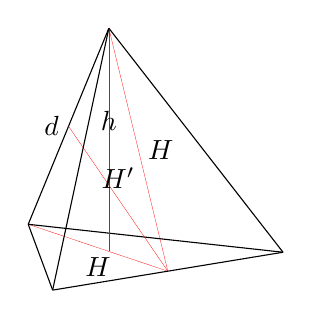
\begin{tikzpicture}[line join=round]
\draw[line width=.1pt,draw=red](-2.055,-1.034)--(-.282,-1.63);
\draw(-2.055,-1.034)--(-1.745,-1.87);
\draw(-1.031,1.456)--(-2.055,-1.034);
\draw(-2.055,-1.034)--(1.181,-1.389);
\draw[line width=.1pt,draw=red](-.282,-1.63)--(-1.543,.211);
\draw[line width=.1pt,draw=red](-1.031,1.456)--(-1.031,-1.378);
\draw(1.181,-1.389)--(-1.031,1.456);
\draw(1.181,-1.389)--(-1.745,-1.87);
\draw(-1.745,-1.87)--(-1.031,1.456);
\draw[line width=.1pt,draw=red](-1.031,1.456)--(-.282,-1.63);
\node[below] at (-1.169,-1.332) {$H$};\node[right] at (-.657,-.087) {$H$};\node[above] at (-1.031,.039) {$h$};\node[above] at (-.913,-.709) {$H'$};\node[left] at (-1.543,.211) {$d$};\end{tikzpicture}% End sketch output

\end{center}

What we are trying to find is $d$ as a function of $h$. Since $H$, $d/2$ and $d$ create a right angeled triangle, it follows
thae $H^2+(d/2)^2=d^2$ and so $H=\sqrt{3}/2d$. Since the size of the inner triangle could be computed two ways then $hH=dH'$ and
since $H'=\sqrt{H^2-(d/2)^2}$ it follows after some math that $d=\sqrt{3/2}h$ which makes $d$ about $1.224h$.

The solution built on this analysis will look like this:

\begin{center}
% Sketch output, version 0.3 (build 7d, Wed May 2 06:36:52 2012)
% Output language: PGF/TikZ,LaTeX
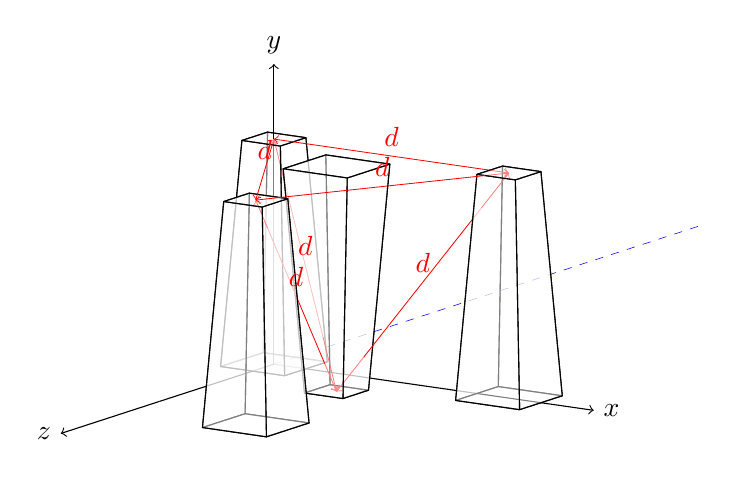
\begin{tikzpicture}[line join=round]
\draw[line width=.2pt,draw=blue,dashed](-2.437,-.792)--(2.708,.88);
\filldraw[fill opacity=0.5,fill=white](-2.031,-.85)--(-2.843,-.733)--(-2.789,2.067)--(-2.302,1.997)--cycle;
\filldraw[fill opacity=0.5,fill=white](-2.843,-.733)--(-3.385,-.909)--(-3.114,1.962)--(-2.789,2.067)--cycle;
\draw[line width=.2pt,draw=blue,dashed](-2.708,-.88)--(-2.437,-.792);
\draw[arrows=-](-2.708,-.88)--(-2.302,-.938);
\filldraw[fill opacity=0.5,fill=white](-2.843,-.733)--(-3.385,-.909)--(-2.572,-1.026)--(-2.031,-.85)--cycle;
\draw[line width=.3pt,arrows=->,draw=red](-2.536,1.288)--(-2.708,1.979);
\filldraw[fill opacity=0.5,fill=white](-2.572,-1.026)--(-2.031,-.85)--(-2.302,1.997)--(-2.626,1.891)--cycle;
\draw[arrows=-](-2.708,-.88)--(-2.978,-.968);
\draw[arrows=-](-2.708,-.88)--(-2.708,1.979);
\filldraw[fill opacity=0.5,fill=white](-3.385,-.909)--(-2.572,-1.026)--(-2.626,1.891)--(-3.114,1.962)--cycle;
\draw[line width=.3pt,arrows=<-,draw=red](-2.708,1.979)--(-2.729,1.906);
\filldraw[fill opacity=0.5,fill=white](-2.789,2.067)--(-3.114,1.962)--(-2.626,1.891)--(-2.302,1.997)--cycle;
\draw[arrows=-](-2.302,-.938)--(-1.659,-1.031);
\draw[arrows=-](-2.978,-.968)--(-4.16,-1.352);
\draw[arrows=->](-2.708,1.979)--(-2.708,2.933);
\draw[line width=.3pt,arrows=<-,draw=red](-2.708,1.979)--(-2.464,1.944);
\draw[arrows=-](-1.659,-1.031)--(-1.172,-1.102);
\draw[line width=.3pt,arrows=-,draw=red](-2.464,1.944)--(.033,1.584);
\draw[line width=.3pt,arrows=-,draw=red](-2.084,-.536)--(-2.536,1.288);
\draw[line width=.3pt,arrows=-,draw=red](-2.729,1.906)--(-2.917,1.277);
\draw[arrows=-](-1.172,-1.102)--(-.129,-1.252);
\filldraw[fill opacity=0.5,fill=white](-2.59,1.602)--(-2.048,1.778)--(-1.994,-1.14)--(-2.319,-1.246)--cycle;
\filldraw[fill opacity=0.5,fill=white](-1.507,-1.21)--(-1.831,-1.316)--(-2.319,-1.246)--(-1.994,-1.14)--cycle;
\filldraw[fill opacity=0.5,fill=white](-2.048,1.778)--(-1.236,1.661)--(-1.507,-1.21)--(-1.994,-1.14)--cycle;
\draw[line width=.3pt,arrows=-,draw=red](-.072,1.106)--(-.637,.389);
\filldraw[fill opacity=0.5,fill=white](.142,-1.164)--(-.4,-1.34)--(-.129,1.531)--(.196,1.636)--cycle;
\filldraw[fill opacity=0.5,fill=white](.954,-1.281)--(.142,-1.164)--(.196,1.636)--(.683,1.566)--cycle;
\filldraw[fill opacity=0.5,fill=white](.142,-1.164)--(-.4,-1.34)--(.412,-1.457)--(.954,-1.281)--cycle;
\draw[line width=.3pt,arrows=<-,draw=red](-1.913,-1.228)--(-2.084,-.536);
\draw[line width=.3pt,arrows=->,draw=red](-1.564,-.786)--(-1.913,-1.228);
\filldraw[fill opacity=0.5,fill=white](-1.236,1.661)--(-1.777,1.485)--(-1.831,-1.316)--(-1.507,-1.21)--cycle;
\filldraw[fill opacity=0.5,fill=white](-1.236,1.661)--(-1.777,1.485)--(-2.59,1.602)--(-2.048,1.778)--cycle;
\draw[line width=.3pt,arrows=->,draw=red](-2.062,-.874)--(-1.913,-1.228);
\filldraw[fill opacity=0.5,fill=white](-1.777,1.485)--(-2.59,1.602)--(-2.319,-1.246)--(-1.831,-1.316)--cycle;
\draw[arrows=-](-.129,-1.252)--(.683,-1.369);
\draw[line width=.3pt,arrows=-,draw=red](-.999,-.069)--(-1.564,-.786);
\filldraw[fill opacity=0.5,fill=white](.412,-1.457)--(.954,-1.281)--(.683,1.566)--(.358,1.461)--cycle;
\draw[line width=.3pt,arrows=-,draw=red](-2.789,.85)--(-2.062,-.874);
\draw[line width=.3pt,arrows=-,draw=red](-.637,.389)--(-.999,-.069);
\draw[line width=.3pt,arrows=<-,draw=red](.277,1.548)--(-.072,1.106);
\filldraw[fill opacity=0.5,fill=white](-.4,-1.34)--(.412,-1.457)--(.358,1.461)--(-.129,1.531)--cycle;
\draw[arrows=->](-4.16,-1.352)--(-5.415,-1.76);
\draw[line width=.3pt,arrows=->,draw=red](.033,1.584)--(.277,1.548);
\draw[line width=.3pt,arrows=<-,draw=red](.277,1.548)--(-.026,1.516);
\filldraw[fill opacity=0.5,fill=white](.196,1.636)--(-.129,1.531)--(.358,1.461)--(.683,1.566)--cycle;
\draw[arrows=->](.683,-1.369)--(1.354,-1.466);
\draw[line width=.3pt,arrows=-,draw=red](-.026,1.516)--(-.248,1.492);
\draw[line width=.3pt,arrows=-,draw=red](-.248,1.492)--(-1.157,1.395);
\filldraw[fill opacity=0.5,fill=white](-2.262,-1.626)--(-3.074,-1.509)--(-3.02,1.292)--(-2.532,1.222)--cycle;
\filldraw[fill opacity=0.5,fill=white](-3.074,-1.509)--(-3.615,-1.684)--(-3.345,1.186)--(-3.02,1.292)--cycle;
\filldraw[fill opacity=0.5,fill=white](-3.074,-1.509)--(-3.615,-1.684)--(-2.803,-1.802)--(-2.262,-1.626)--cycle;
\draw[line width=.3pt,arrows=-,draw=red](-1.157,1.395)--(-2.494,1.252);
\draw[line width=.3pt,arrows=<-,draw=red](-2.939,1.204)--(-2.789,.85);
\filldraw[fill opacity=0.5,fill=white](-2.803,-1.802)--(-2.262,-1.626)--(-2.532,1.222)--(-2.857,1.116)--cycle;
\filldraw[fill opacity=0.5,fill=white](-3.615,-1.684)--(-2.803,-1.802)--(-2.857,1.116)--(-3.345,1.186)--cycle;
\filldraw[fill opacity=0.5,fill=white](-3.02,1.292)--(-3.345,1.186)--(-2.857,1.116)--(-2.532,1.222)--cycle;
\draw[line width=.3pt,arrows=->,draw=red](-2.917,1.277)--(-2.939,1.204);
\draw[line width=.3pt,arrows=-,draw=red](-2.494,1.252)--(-2.635,1.237);
\draw[line width=.3pt,arrows=->,draw=red](-2.635,1.237)--(-2.939,1.204);
\node[right] at (1.354,-1.466) {$x$};\node[above] at (-2.708,2.933) {$y$};\node[left] at (-5.415,-1.76) {$z$};\node[above,color=red] at (-2.823,1.592) {$d$};\node[above,color=red] at (-.818,.16) {$d$};\node[above,color=red] at (-1.215,1.764) {$d$};\node[above,color=red] at (-1.331,1.376) {$d$};\node[above,color=red] at (-2.426,-.012) {$d$};\node[above,color=red] at (-2.31,.376) {$d$};\end{tikzpicture}% End sketch output

\end{center}

As is evident the key to solving this question is the perfect triangular pyramid as both solutions are based on it and it is the only
way to put 4 elements in space being spaced equally apart. In theory you could place the bottles at any height and so
infinite solutions to this riddle could be produced by making the side of the perfect pyramid as small or as large as you want. But we are
constrained by the table and so the heights at which the caps are will be either $0$ or $h$. The two solutions above seem to be primary
examples under this constraint. Minor variations on the above two solutions could be produced by making the bottles whose caps are at table
level lay instead of stand on their heads. The first solution is more attractive than the second because it could be performed in practice
without relying on measurement tools in order to place the bottles at the calculated distance from each other as per the second solution.

\section{Strange Trip (Geometry)}
You travel 100 miles north, 100 miles east, and then 100 miles south. You are at the same point that you started from. Describe all the places on earth this could be, if any.

\subsection{Solution}
At the south pole. Or, 100 miles south of any point on the circle around the north pole that is 100 miles in circumference. Or, 100 miles south of any such circle whose circumference is an integral fraction of 100 miles.

\section{Three Cards (Probability)}
There are 3 cards: one is all red, one is all blue, and the third is blue on one side and red on the other. The cards are shuffled. You pick one at random and it is blue on the side facing you. What are the chances that it is also blue on the other side?

\subsection{Solution}
2/3. 2 of the 3 blue sides have blue on the other side. You might think the odds are 50/50 because you could have one of two cards, but you actually get a side at random, not a card, so you are more likely to have the blue/blue card than the red/blue card.

Here is another way to think of it: When you pick a card at random, the chances of it being the same on both sides (either all red or all blue) are 2 out of 3, and this doesn't change just because you see one of the sides. If they did, they'd change no matter which color you saw, and it wouldn't even matter if you looked. So when you do see the blue side, the red/red card is eliminated, but the blue/blue card still has a 2/3 probability.

\section{Monty Hall Problem (Probability)}
Behind 1 of 3 closed doors is a prize. You pick one of the doors. Monty opens one of the other doors and it is empty. You are given the choice of sticking with your choice or switching to the other unopened door. Should you switch? What are your chances of winning if you do?

\subsection{Solution}
You should switch. Your chances are 2/3 if you do. The initial chances of your first choice were 1/3, and opening another door without the prize doesn't actually change that, so the remaining door now has a 2/3 chance because the chances of all possibilities must sum to 1.

Many people think the chances are 50/50 because there are two doors left, but that is not correct. If you're not convinced 2/3 is correct, consider a 100 door version: you pick 1 door and Monty opens 98 other doors avoiding the one with the prize. Now you have a 99\% chance if you switch.

\section{4 Door Monty Hall Problem (Probability)}
Behind 1 of 4 closed doors is a prize. You pick door 1. Monty opens the 4th door and it is empty. You switch your choice to door 2. Now monty opens door 3 and it is also empty. Given the choice, should you switch back to door 1, and what are your chances of winning if you do?

\subsection{Solution}
Yes, your chances are 5/8 if you switch. The initial chances of your first choice were 1/4, and opening another door without the prize doesn't change that, so the remaining 2 doors now have a 3/8 chance because the chances of all possibilities must sum to 1. But then when Monty opens door 3, using the same reasoning, door 2 stays at 3/8 chance and so the remaining door changes to 5/8.

\section{Two Envelopes, Also known as the exchange paradox (Probability)}
There are two envelopes, one contains twice as much money as the other. You pick one at random and find \$100 inside. What is the "expected value" of the amount in the other envelope? Given the option, should you switch? Does it matter how much you found in that first envelope? Does it matter if you open the envelope?

\subsection{Solution}
This is a strange paradox because it appears that the expected value is the average of double and half which is 1.25 X so you should switch. However, this would be true for any value of X you find, so it wouldn't even matter if you open the envelope. This same logic suggests that you should also immediately switch back to the original envelope again, which doesn't make sense at all.

The fault in this reasoning is that you are not actually given enough information to know that double and half are equally probable. You would need to know more about the process by which the amounts in the envelopes were determined or what the probability distribution of possible amounts is. For example, if there was a known limit for the amounts, you would switch if and only if 2X was within that limit. Note that it is impossible to have an even distribution of all possible values without also having an upper bound. If the amounts can go to infinity, there would have to be some uneven probability distribution, and you would need to know what that was to solve the problem properly.

Given the lack of any information like this, I believe the correct answer is: It does not matter if you switch.

\section{100 urns (Mathematics)}
There's a room with 100 urns, 2 people standing outside, while they decide on what to do 100 balls are randomly placed inside the urns. one of the people from outside will enter the room, be given the placement of all the balls, look at it and switch two balls from among the 100 balls, then he will be whisked away to a vacation in Mali. The other one will then enter, be given a random number for a ball to be found. He needs to find it while breaking (checking) as few urns as possible. What is the strategy?
Hint: this can be done with 50 urns broken or less.

\subsection{Solution}
Lets give a solution which is not good, analyze it and then improve it.
Here is the bad solution. Whenever the second person comes in he is given the task of finding the ball marked $x$. He will proceed to break urn $x$. If $x$ is there he is done. If not, then some other ball $y$ is there. He will process to do the same for $y$.

Analysis: Can the second person get stuck in an infinite loop? No. There are only 100 urns so in the worst case scenario he will break all 100 urns and find the ball $x$ in the last one. Now lets take this further. Lets define an equivalence relation on the urns: two urns $x$ and $y$ are equivalent if there exists a route from $x$ to $y$. This is indeed an equivalence relation since there is always a route from $x$ to $x$. If there is a route from $x$ to $y$ then there is also a route from $y$ to $x$ since in our case there is only one route to each urn (only one urn carries the ball with it's number). Since starting a route from $y$ must eventually lead back to $y$ (routes do not just end), it must pass through $x$. All this means is that our 100 urns are divided into cycles of equivalence.

Now for the first players job. When the first player comes along he will either see all cycles with $size<=50$ in which case he need not do anything (unless he wants to break up the largest cycle to reduce the expected value of urns broken by the second player) or will be confronted with utmost a single cycle with $size > 50$ which means he needs to break just this one cycle.

How does one go about "breaking" a cycle? A cycle is a list of urns $x_1, x_2, ...,x_{n-1} ,x_n$ that make up a cycle, which means their content is $x_2, x_3,..., x_n, x_1$. In order to break the cycle you need to find the center of the cycle. If the length of the cycle is odd then the center is the middle element if the lengh is even pick any of the central two elements. In our case the longest cycle cannot be of length greater than $100$ which means that breaking it up in the center will  break it up to pieces less or equal to 50. Lets say the center is in urn $k$. Switch the content of urns $k$ and $n$. This will create two cycles: $x_1, x_2, ... , x_k$ with content $x_2, x_3, ... , x_1$ and another cycle $x_{k+1}, x_{k+2}, ... , x_n$ with content $x_{k+2}, x_{k+3}, ... , x_{k+1}$.

\section{Blue and red martians (Distributed algorithms)}
On mars live two types of aliens: ones with blue dots on their head and ones with blue dots. No martian knows what color dot he/she has on their head and they do not have verbal skills. One day they get told that a new virus is out there that only kills the blue kind and therefor all the blue martians must leave the planet to space where the virus cannot survive. Red martians, however, must not leave the planet since they cannot survive in outer space. Each day a ship, large enough to hold all the martians, will leave at noon carrying martians to outer space. Can just the blue martians leave? if so how? p.s. there is at least one martian with a blue dot on his head and everyone knows so.

\subsection{Solution}
Since the martians are very smart, if there are $N$ martians then all of them will leave on day $N$. How is that? The proof is by induction. Imagine that there is only one martian with a blue dot. He sees everyone with red dots on their head and since he knows that there is at least one martian with a blue dot on his/her head he deduces that it is he. He therefor leaves in the first possible occasion, meaning the first day. Now imagine that the proposition is true for $N$. Now imagine that there are $N+1$ martians. Each of them sees only $N$ blue dots in the crowd. The deduce that there are either $N$ martians with blue dots (excluding themselves) or $N+1$ blue dotted martians (including themselves). They don't know which. So they wait for day $N$. If there were indeed $N$ martians all of them would have left on day $N$. They do not leave. From this each one of the $N+1$ deduces that the other $N$ martians see $N$ blue dots in the crowd which means that they themselves are blue dotted which means that there are $N+1$ blue dotted martians which include themselves. This prompts them to leave on the first possible occasion, which is day $N+1$.

\section{The Wardens challenge (Distributed algorithms)}
A warden summons all of his prisoners to a talk. "From this day on you will not see each other. I will select, by random and with possible repetitions, one of you each day and will place him or her in a special holding chamber. The holding chamber has a light bulb with a switch. When the day is done I will lead the prisoner back to his or her cell. At any time, any one of who understands that all of you have been in the special holding cell may callout and stop the experiment. If that person is right the you will all go free and if he is wrong you will stay here for life". The prisoners then have time to confer and plan a strategy before they are taken to their cells and are prevented from speaking to one another for the remainder of the experiment. Plan the prisoners strategy.

\subsection{Solution}
A first solution would be to use a special designated person to act as counter. The counter never flips the light switch on. Every time the counter is called into the holding cell and sees the light he/she adds $1$ to a sum he/she is storing in memory as to the number of people that have been in the holding cell and flips the light off. Every other prisoner will follow the following rules: If you have never flipped the switch on and the switch is off when you enter the room then switch it on. Otherwise do nothing. The counter is the only person to proclaim that everyone has been to the holding cell and obviously has to count himself/herself as well.

The problem with this solution is that it's efficiency is quite low. Time is also wasted when a prisoner that has never been to the cell enters it and sees the light on which prevents him from turning the light on himself and makes him wait for the next time he/she is called to the holding cell.

\section{Jumping frogs (Geometric)}
Four frogs are sitting on the vertices of a square the side of which is of length $1$. In turns, a frog may lep over any other frog jumping twice the distance between them. Could the frogs, after any number of steps, form a square of a size different than $1$? Another version would be: can you prove that if, after any number of jumps, the frogs form a square then the size of the square will be $1$?

\subsection{Solution}
If we put the frogs on an infinite grid of size $1$ then after each jump all frogs must be located on that grid. So if the frogs can create a square of a size bigger than $1$ then that size must be a whole number which is bigger than $1$. Now lets note that if the frogs can create a square bigger than $1$ then, starting from that square, then can reverse their steps and create a square which is of size $1$. This means that the frogs can make the square they form bigger or smaller by some factor at any time. The problem with this is that this is also true for the original sized $1$ square: the frogs can make it smaller by that same factor but that is a contradiction to the fact that the frogs always remain on the grid.

\label{end}\end{document}
